\input{../../common/slide-common-header.tex}

\newcommand{\orgNum}{0}
\newcommand{\orgTopic}{org meeting}
\newcommand{\orgKey}{syllabus, contacts}

\newcommand{\introNum}{1}
\newcommand{\introTopic}{introduction to multithreading}
\newcommand{\introKey}{concurrency, parallelism, agents, threads, scheduler, Amdahl's law, race condition, deadlock, wait-for graph}

\newcommand{\basicNum}{2}
\newcommand{\basicTopic}{basic concepts}
\newcommand{\basicKey}{mutex, acquisition order, reentrancy, fairness, data locking, code locking, signalling, condition variable, lost signal, spurious wakeup}

\newcommand{\syncPrimitivesNum}{3}
\newcommand{\syncPrimitivesTopic}{advanced synchronization primitives}
\newcommand{\syncPrimitivesKey}{monitor, latch, barrier, thundering herd, semaphore, read-write lock, thread pool, executor, producer-consumer, fork-join, load balancing}

\newcommand{\patternsNum}{4}
\newcommand{\patternsTopic}{advanced synchronization concepts}
\newcommand{\patternsKey}{interruption, cancellation, partitioning, privatization, replication, thread-local, ownership}

\newcommand{\extraBasicsNum}{5}
\newcommand{\extraBasicsTopic}{additional topics of practical concurrency}
\newcommand{\extraBasicsKey}{documenting protocols and classes, checking concurrent invariants, stress testing, execution trace analysis, estimating required testing effort, static and dynamic checks, scheduling randomization, model checking}

\newcommand{\foundationsNum}{6}
\newcommand{\foundationsTopic}{theoretical foundations of concurrency}
\newcommand{\foundationsKey}{timeline, events, precedence, 2-thread mutual exclusion, deadlock freedom, starvation freedom, N-thread mutual exclusion, sequential objects and specifications, concurrent objects, linearizability}

\newcommand{\foundationsPlusNum}{7}
\newcommand{\foundationsPlusTopic}{progress guarantees, concurrent operations hierarchy, consensus number}
\newcommand{\foundationsPlusKey}{obstruction-free, lock-free, wait-free, safe register, regular register, atomic register, register snapshot, consensus number}

\newcommand{\atomicsNum}{8}
\newcommand{\atomicsTopic}{introduction to atomics}
\newcommand{\atomicsKey}{read-modify-write, get-and-add, compare-and-swap, spin lock, lock-free stack, ABA problem}

% TODO: taxonomy of queues, 

\newcommand{\cacheCoherencyNum}{9}
\newcommand{\cacheCoherencyTopic}{cache coherency}
\newcommand{\cacheCoherencyKey}{cache memory hierarchy, cache coherency protocol. store-buffer, load-buffer, invalidate-queue, memory barrier, hardware memory model, weak memory model, litmus tests}

\newcommand{\langMMNum}{10}
\newcommand{\langMMTopic}{language memory model}
\newcommand{\langMMKey}{motivation, approaches, comparison of existing solutions}

\newcommand{\advancedConcurrencyNum}{11}
\newcommand{\advancedConcurrencyTopic}{advanced concurrency}
\newcommand{\advancedConcurrencyKey}{CLH/MCS queue/lock, backoff policies revisited, notify-as-ready, RAT optimization, single LIFO cell optimization, work distribution, work stealing, taxonomy of parallel problems}

\newcommand{\userSpaceThreadingNum}{12}
\newcommand{\userSpaceThreadingTopic}{user-space threading}
\newcommand{\userSpaceThreadingKey}{berkley socket, blocking and non-blocking IO, callback-hell, async-await, continuation-passing-style, fibers/coroutines/green threads, stackful vs stackless}


\newcommand{\designNum}{13}
\newcommand{\designTopic}{designing concurrent systems}
\newcommand{\designKey}{park/unpark, synchronizer, futex/wait-on-address, plan9 approach, race-finders, ForkJoinPool/CoroutineCarriers/UIthread, observability, structured concurrency}

\newcommand{\frameworksAndDistributedNum}{14}
\newcommand{\frameworksAndDistributedTopic}{multi-agent systems}
\newcommand{\frameworksAndDistributedKey}{auto-parallelization languages and frameworks, semi-automatic synchronization, distributed systems, consensus protocols}


\title[]{Lecture \cacheCoherencyNum: \cacheCoherencyTopic}
\subtitle[]{\cacheCoherencyKey}

\author[]{Alexander Filatov\\ filatovaur@gmail.com}
\date{}

\begin{document}

\begin{frame}
  \titlepage
  \url{https://github.com/Svazars/parallel-programming/blob/main/slides/pdf/l9.pdf}
\end{frame}


\begin{frame}{In previous episodes}

Concurrency domain
\begin{itemize}
 \item Communicating agents (threads)
 \item Different speed of execution and non-deterministic interleavings (OS scheduler)
 \item Problems with proper synchronization -- race conditions, deadlocks
 \item Key properties: Safety (correctness), Liveness (progress), Performance
\end{itemize}

Formalization of concurrent execution
\begin{itemize}
 \item Timeline, Events, Intervals, Precedence
 \item Consistency, Linearizability, Linearization points
 \item Progress conditions: wait-free, lock-free, obstruction-free, starvation-free, deadlock-free
 \item Atomic register, Snapshot, Consensus number
\end{itemize}

Practical aspects
\begin{itemize}
 \item Read-Modify-Write operations
 \item Memory bus, Cache hierarchy, Cache coherence
 \item Lock-free algorithms and ABA problem
\end{itemize}
\end{frame}

\begin{frame}{Warning: lecture today is going to be like}

\pause

\begin{tikzpicture}[remember picture,overlay]
\node[xshift=4cm,yshift=1cm] at (current page.center) {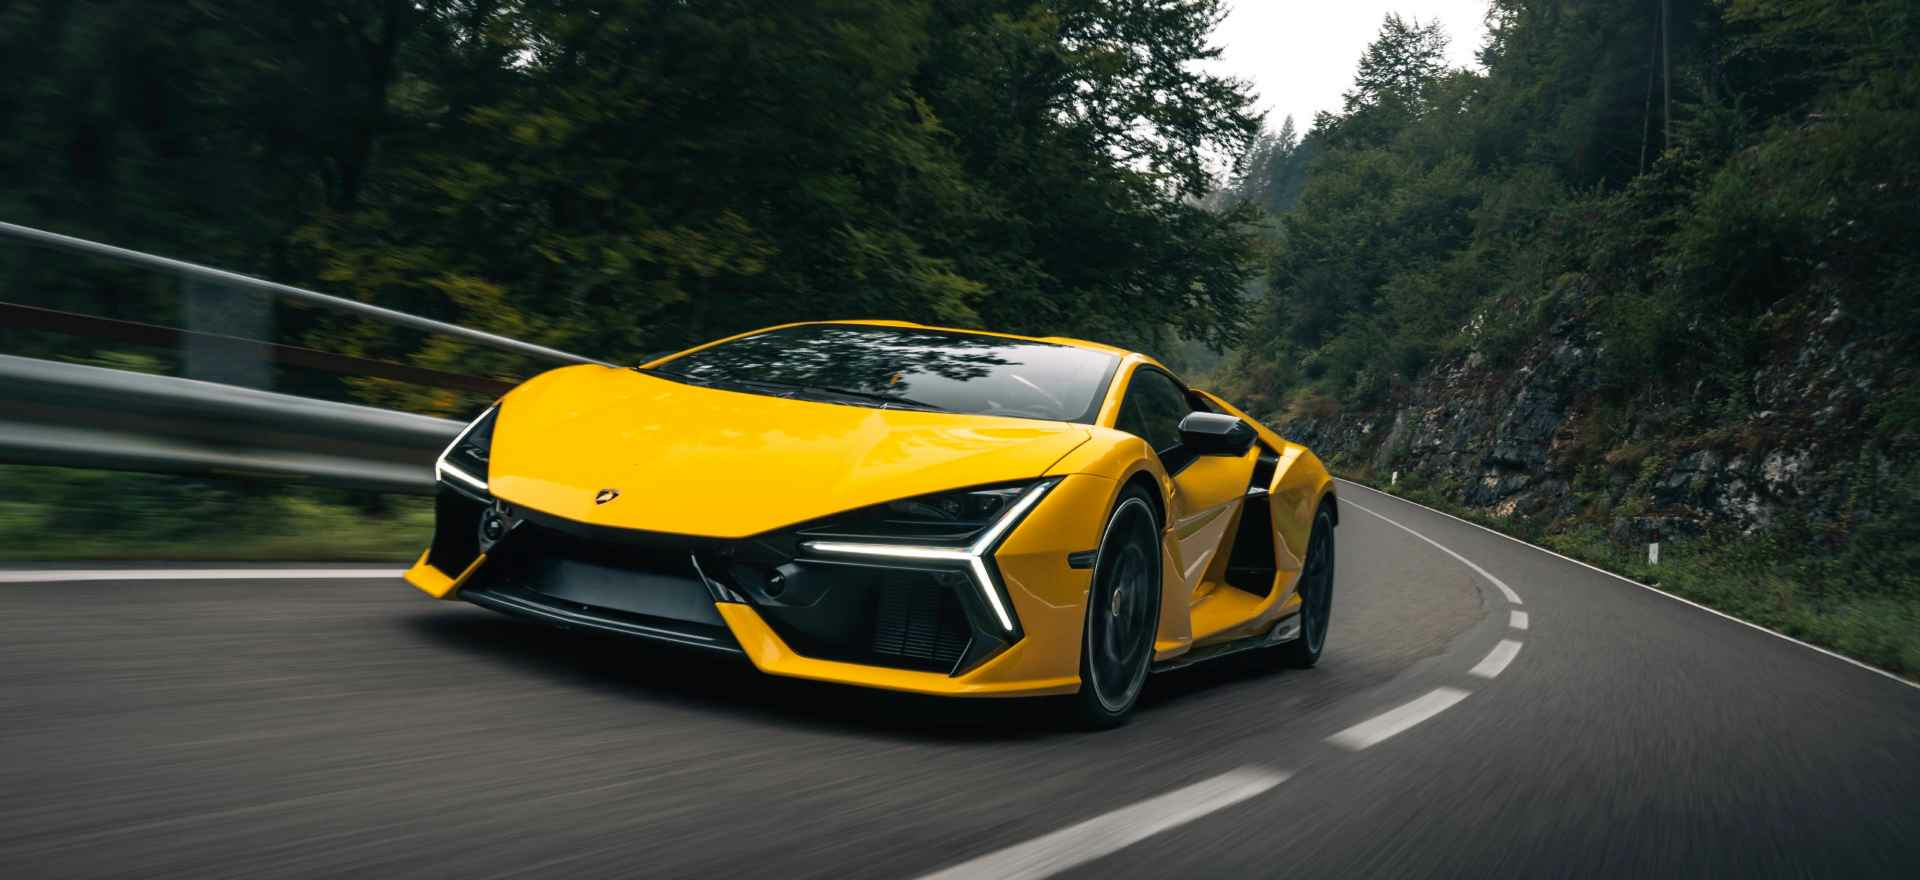
\includegraphics[width=0.4\textwidth]{./pics/lambo.png}};
\end{tikzpicture}

\pause

\begin{tikzpicture}[remember picture,overlay]
\node[xshift=-5cm,yshift=-0cm] at (current page.center) {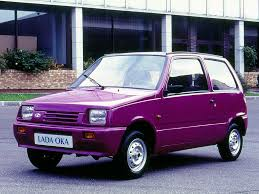
\includegraphics[width=0.3\textwidth]{./pics/oca.png}};
\end{tikzpicture}

\pause

\begin{tikzpicture}[remember picture,overlay]
\node[xshift=1cm,yshift=-2cm] at (current page.center) {
\includegraphics[width=0.3\textwidth]{./pics/prof.png}};
\end{tikzpicture}

\end{frame}

\begin{frame}{Supplementary materials}

Unconditional benefit
\begin{itemize}
  \item "Memory Barriers: a Hardware View for Software Hackers"\footnote{\tiny\url{https://www.researchgate.net/publication/228824849_Memory_Barriers_a_Hardware_View_for_Software_Hackers}}
  \item "What Every Programmer Should Know About Memory"\footnote{\tiny\url{https://people.freebsd.org/~lstewart/articles/cpumemory.pdf}}
  \item "Слабые модели памяти: буферизации записи на x86"\footnote{\tiny\url{https://habr.com/ru/companies/JetBrains-education/articles/523298}}
\end{itemize}

Advanced material
\begin{itemize}
  \item "A Tutorial Introduction to the ARM and POWER Relaxed Memory Models"\footnote{\tiny\url{https://www.cl.cam.ac.uk/~pes20/ppc-supplemental/test7.pdf}}
  \item "Shared Memory Consistency Models: A Tutorial"\footnote{\tiny\url{https://dl.acm.org/doi/10.1109/2.546611}}
\end{itemize}

Mechanical sympathy (better understand h/w design):
\begin{itemize}
  \item "Digital Design and Computer Architecture" \ by David Money Harris, Sarah L. Harris\footnote{\tiny\url{https://www.amazon.com/Digital-Design-Computer-Architecture-Harris/dp/0123944244}}
\end{itemize}

\end{frame}


\begin{frame}{Lecture plan}
\tableofcontents
\end{frame}


\section{Preliminary discussion}


\begin{frame}{Global memory: 1 CPU}

\begin{center}
  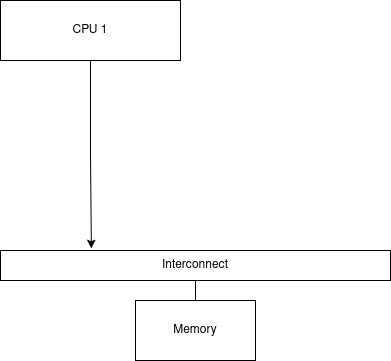
\includegraphics[width=0.3\textwidth]{./pics/processor/1.png}
\end{center}

\end{frame}

\begin{frame}[t]{Global memory: 2 CPU}

\begin{center}
  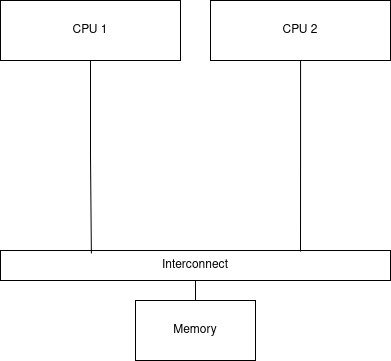
\includegraphics[width=0.3\textwidth]{./pics/processor/2.png}
\end{center}

\pause

Any problem here?

\end{frame}

\begin{frame}[t,noframenumbering]{Global memory: 2 CPU}

\begin{center}
  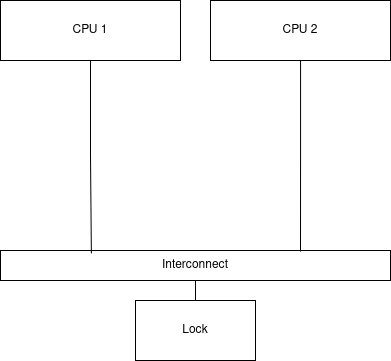
\includegraphics[width=0.3\textwidth]{./pics/processor/3.png}
\end{center}

\pause

Any problem here?

\end{frame}



\begin{frame}[t]{Global memory: fine-grained locking}

\begin{center}
  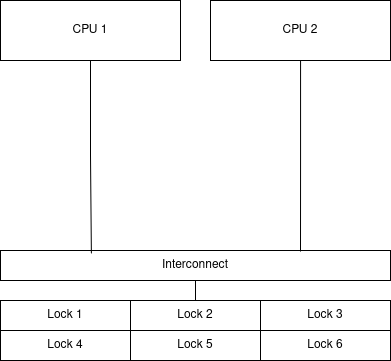
\includegraphics[width=0.3\textwidth]{./pics/processor/4.png}
\end{center}

\pause

Cache line
\begin{itemize}
    \item contiguous chunk of memory (e.g 64, 128, 256 bytes)
    \item auxiliary data associated with the chunk
\end{itemize}

\end{frame}


\begin{frame}[t, noframenumbering]{Global memory: fine-grained locking}

\begin{center}
  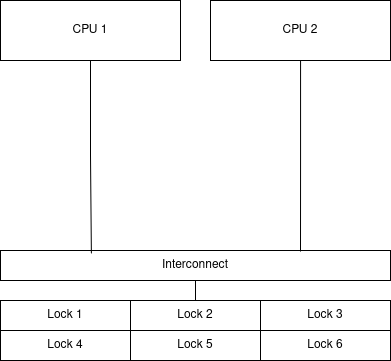
\includegraphics[width=0.3\textwidth]{./pics/processor/4.png}
\end{center}


What is optimal cache line size?

\pause
\begin{itemize}
    \item too large -- \textbf{false sharing} (access to independent data cause performance loss)
    \item too small -- overhead for storing meta information
\end{itemize}    

\end{frame}


\begin{frame}[t, noframenumbering]{Global memory: fine-grained locking}

\begin{center}
  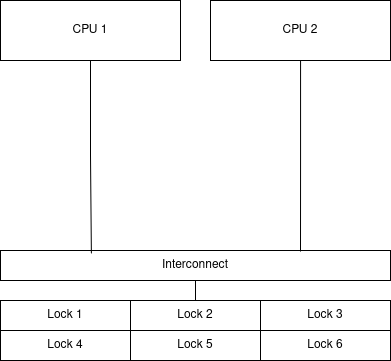
\includegraphics[width=0.3\textwidth]{./pics/processor/4.png}
\end{center}

Any problem here?

\end{frame}


\begin{frame}{Global memory: fine-grained locking for read-mostly data}

\begin{center}
  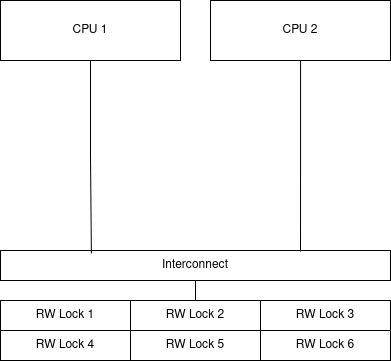
\includegraphics[width=0.3\textwidth]{./pics/processor/5.png}
\end{center}

\pause

Is it consistent?

\end{frame}

\begin{frame}{Global memory: fine-grained locking for read-mostly data}

\begin{center}
  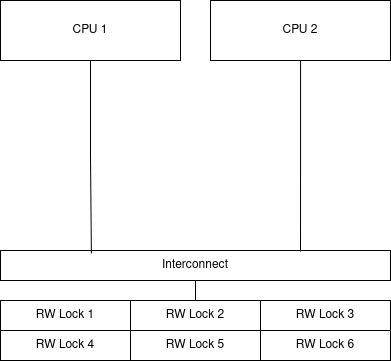
\includegraphics[width=0.3\textwidth]{./pics/processor/5.png}
\end{center}

\begin{itemize}
    \item \textbf{Coherence}: in any execution, for each location, there is a single linear order of all writes to that location which must be respected by all threads
\end{itemize}

\pause
What?

\end{frame}

\begin{frame}[t,fragile]{Coherency: CoRR1 sample}

\begin{itemize}
    \item \textbf{Coherence}: in any execution, for each location, there is a single linear order of all writes to that location which must be respected by all threads
\end{itemize}

\pause

Initial state: \texttt{x = 1}
\begin{tabular}{p{0.5\textwidth} p{0.5\textwidth}} 
 \begin{minted}[fontsize=\small]{c}
 void threadA() {
       x = 2;   
 }
 \end{minted}
 &  
 \begin{minted}[fontsize=\small]{c}
 void threadB() {                                   
     int r1 = x;                           
     int r2 = x;                           
 }                    
 \end{minted}
\end{tabular}

\pause
\texttt{Forbidden: r1 = 2, r2 = 1}

\pause
Several other executions of the same code are allowed: 
\begin{itemize}
    \item both Thread B reads could read 1
    \item both Thread B reads could read 2
    \item first could read 1 and the second 2
\end{itemize}

\end{frame}


\begin{frame}[t,fragile]{Coherency: CoRR2 sample}

\begin{itemize}
    \item \textbf{Coherence}: in any execution, for each location, there is a single linear order of all writes to that location which must be respected by all threads
\end{itemize}

\pause

Initial state: \texttt{x = 0}
\begin{tabular}{p{0.2\textwidth} p{0.2\textwidth} p{0.2\textwidth} p{0.2\textwidth}}
 \begin{minted}[fontsize=\small]{python}
 thread1
   x = 1
 \end{minted}
 
 & 
 
 \begin{minted}[fontsize=\small]{python}
 thread2
   x = 2
 \end{minted}
 
 &
 
 \begin{minted}[fontsize=\small]{python}
 thread3
  r1 = x
  r2 = x 
 \end{minted}
 
 &
 
 \begin{minted}[fontsize=\small]{python}
 thread4
  r3 = x
  r4 = x
 \end{minted}
 \end{tabular}
 

\pause
\texttt{Forbidden: r1 = 2, r2 = 1, r3 = 1, r4 = 2}

\end{frame}


\begin{frame}{Global memory: fine-grained locking for read-mostly data}

\begin{center}
  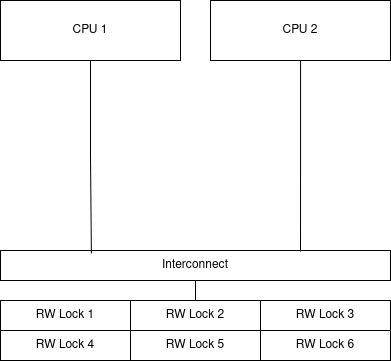
\includegraphics[width=0.3\textwidth]{./pics/processor/5.png}
\end{center}

\begin{itemize}
    \item \textbf{Coherence}: in any execution, for each location, there is a single linear order of all writes to that location which must be respected by all threads
\end{itemize}

\pause

What about two locations?
\pause
\begin{itemize}
    \item No ordering required, no linearizability assumed
\end{itemize}

\pause

What?

\end{frame}

\begin{frame}[t,fragile]{Coherency is about single memory cell}

\begin{itemize}
    \item \textbf{Coherence}: in any execution, for each location, there is a single linear order of all writes to that location which must be respected by all threads
\end{itemize}

\pause

Initial state: \texttt{x = 1, y = 1}
\begin{tabular}{p{0.3\textwidth} p{0.3\textwidth} p{0.3\textwidth}} 
 \begin{minted}[fontsize=\small]{c}
 void threadA() {
       x = 2;   
       y = 2;
 }
 \end{minted}
 &  
 \begin{minted}[fontsize=\small]{c}
 void threadB() {                                   
     int r1 = x;                           
     int r2 = y;                           
 }
 \end{minted}
 &
 \begin{minted}[fontsize=\small]{c}
 void threadC() {                                   
     int r3 = y;                           
     int r4 = x;                           
 }                   
 \end{minted}
\end{tabular}

\pause
\texttt{Allowed: r1 = 2, r2 = 1, r3 = 2, r4 = 1}

\pause
\textbf{Important:}
\begin{itemize}
    \item "each location has single linear order of all writes" \ \textbf{does not imply} orders of independent locations are "aligned"
    \pause
    \item \textbf{Coherence} is weaker than linearizability
\end{itemize}

\end{frame}

\begin{frame}[t,fragile]{Idea}

\begin{itemize}
    \item \textbf{Coherence} is weaker than linearizability
\end{itemize}

\pause

Let's reorder independent memory operations to improve performance of the CPU!

\pause
Every single-threaded program will become faster!

\pause
Who cares that concurrent software will misbehave, right?

\end{frame}


\begin{frame}[t,fragile]{Relaxing memory ordering guarantees}

\begin{minted}{java}
static int x, y;
void foo() {
  int r1 = x;
  int r2 = y;
}
\end{minted}

\end{frame}


\begin{frame}[t,fragile,noframenumbering]{Relaxing memory ordering guarantees}

\begin{minted}{java}
static int x, y;
void foo() {
  int r1 = memory.read(x);
  int r2 = memory.read(y);
}
\end{minted}

\pause

\begin{tikzpicture}[remember picture,overlay]
\node[xshift=0cm,yshift=-6.5cm] at (current page.center) {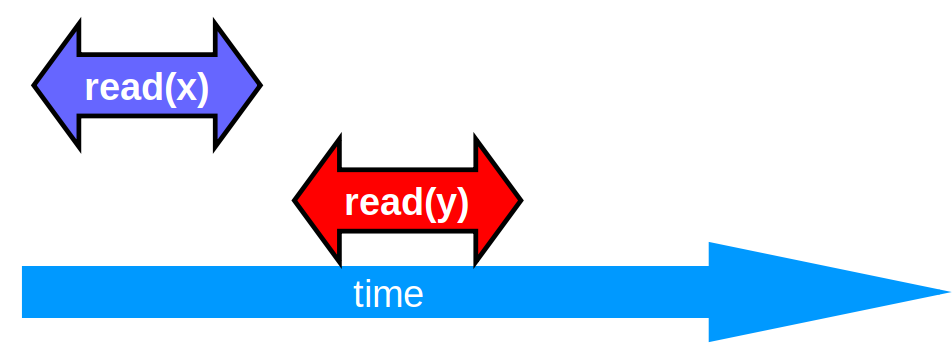
\includegraphics[width=0.5\textwidth]{./pics/reorder1.png}};
\end{tikzpicture}

\end{frame}


\begin{frame}[t,fragile,noframenumbering]{Relaxing memory ordering guarantees}

\begin{minted}{java}
static int x, y;
void foo() {
  Future<int> r1 = memory.read(x);
  Future<int> r2 = memory.read(y);
}
\end{minted}

\end{frame}


\begin{frame}[t,fragile,noframenumbering]{Relaxing memory ordering guarantees}

\begin{minted}{java}
static int x, y;
void foo() {
  Future<int> r1 = memory.read(x);
  Future<int> r2 = memory.read(y);
  ...

  use(r2.get());
  ...
  use(r1.get());
}
\end{minted}

\pause

\begin{tikzpicture}[remember picture,overlay]
\node[xshift=3cm,yshift=-2.5cm] at (current page.center) {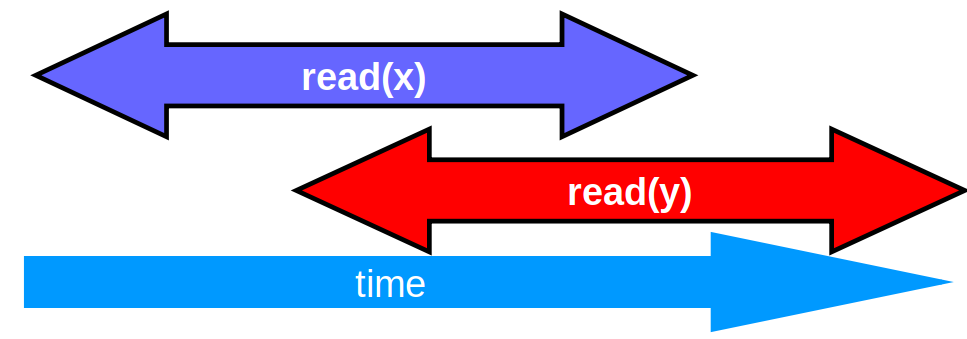
\includegraphics[width=0.5\textwidth]{./pics/reorder2.png}};
\end{tikzpicture}

\end{frame}


\begin{frame}[t,fragile,noframenumbering]{Relaxing memory ordering guarantees}

\begin{minted}{java}
static int x, y;
void foo() {
  Future<int> r1 = memory.read(x);
  Future<int> r2 = memory.read(y);
  ...

  use(r2.get());
  ...
  use(r1.get());
}
\end{minted}

\begin{itemize}
    \item Improve efficiency and CPU utilization -- faster
    \item Sacrifice consistency -- harder to reason about correctness
\end{itemize}

\end{frame}


\begin{frame}{Implementing hardware memory: challenges}

\begin{itemize}
    \item Provide efficient and scalable hardware implementation of shared memory
    \pause
    \item Maintain consistency of single memory cell -- \textbf{coherency}
    \pause
    \item Allow to reorder operations on independent memory cells -- \textbf{relaxed memory model}
\end{itemize}

\pause
Our plan:
\begin{itemize}
    \pause
    \item Look at simplified model: replication pattern for cache lines + MESI protocol
    \pause
    \item Improve it: Store buffering, Load buffering, Invalidate queue, Interconnect topology    
    \pause
    \item Repair multi-cell consistency using memory barriers
    \pause
    \item Empirically study concurrent behaviour of existing hardware via litmus tests
\end{itemize}

\end{frame}

\section{Cache coherency}
\showTOC

\begin{frame}{Why do we need caches?}

\pause

\begin{center}
    \textbf{Nanoseconds and toilet paper show}
\end{center}

\pause

\begin{center}
   \url{https://travisdowns.github.io/blog/2020/07/06/concurrency-costs.html}

   Level 2 (True Sharing)
\end{center}


\end{frame}


\begin{frame}{Using caches}

\begin{center}
  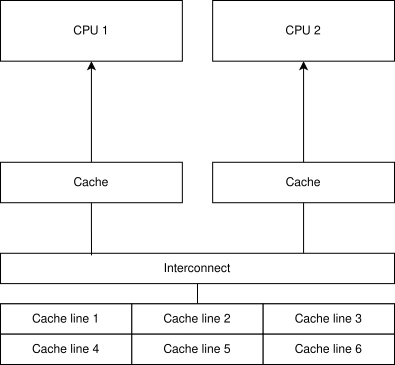
\includegraphics[width=0.3\textwidth]{./pics/processor/cache.png}
\end{center}

Replication pattern:
\begin{itemize}
    \item Cache line copied to processor-local cache
    \item Metadata associated with every replicated cache line -- state of cache line
\end{itemize}
\end{frame}

\begin{frame}{Homework: caches and associativity}

Hardware caches are quite efficient and use hardware-supported N-way associativity

"Is Parallel Programming Hard, And, If So, What Can You Do About It" \ (perfbook) 
\begin{itemize}
    \item Appendix B "Why Memory Barriers?" \ , section B.1 "Cache Structure"
    \item perfbook.B.1
\end{itemize}

Be ready to draw and explain what is associative hardware cache.

\end{frame}

\begin{frame}{Distributed caching}

\begin{center}
  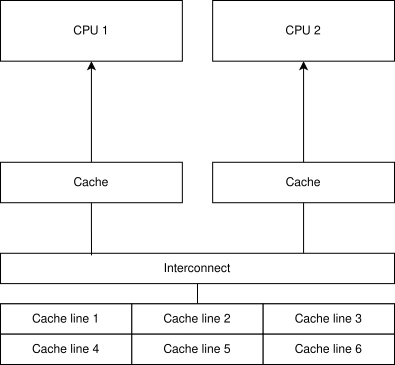
\includegraphics[width=0.3\textwidth]{./pics/processor/cache.png}
\end{center}

\begin{itemize}
    \item \textbf{Coherence}: in any execution, for each location, there is a single linear order of all writes to that location which must be respected by all threads
\end{itemize}

\pause

How to implement that without locks? \pause And without Atomic MRMW registers? \pause Efficient?

\end{frame}


\begin{frame}{Cache coherency: MESI}

\begin{tikzpicture}[remember picture,overlay]
\node[xshift=4cm,yshift=-6.5cm] at (current page.center) {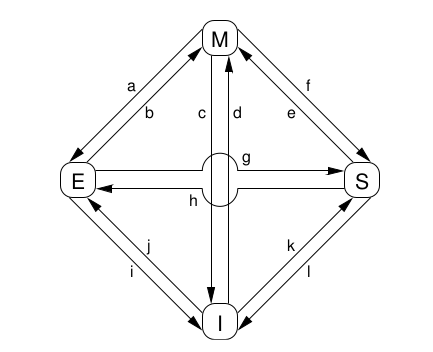
\includegraphics[width=0.5\textwidth]{./pics/MESI.png}};
\end{tikzpicture}


State machine:
\begin{itemize}
    \item \textbf{Modified}
    \item \textbf{Exclusive}
    \item \textbf{Shared}
    \item \textbf{Invalid}
\end{itemize}

Message passing on some transitions:
\begin{itemize}
    \item asynchronous (fire and forget)
    \item synchronous (cannot change state until confirmation received)
\end{itemize}


\end{frame}


\begin{frame}[fragile]{Cache coherency: message passing\footnote{perfbook.B.2.3.}}

\begin{tikzpicture}[remember picture,overlay]
\node[xshift=5cm,yshift=-7.5cm] at (current page.center) {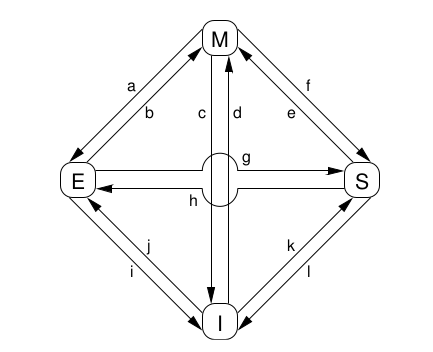
\includegraphics[width=0.4\textwidth]{./pics/MESI.png}};
\end{tikzpicture}


\begin{tabular}{p{10cm}p{5cm}}

\begin{itemize}
    \item Transition \textbf{(k)}: CPU loads data in a cache line that was not in its cache. Send “read”, await “read response”.

    \item Transition \textbf{(h)}: CPU realizes that it will soon need to write data in this cache line. Send “invalidate” message, await "invalidate acknowledge". 

    \item Transition \textbf{(b)}: CPU writes to the cache line that it already had exclusive access to. Nothing to send/receive.

    \item Transition \textbf{(c)}: CPU receives “read invalidate” message for a cache line that it has modified. The CPU must invalidate local copy, respond with “read response” and “invalidate acknowledge”.
\end{itemize}

 &
 
\end{tabular}

\end{frame}

\begin{frame}{Homework: more complicated MESI protocol example}

Homework: read perfbook.B.2.4. "MESI Protocol Example"

\begin{center}
    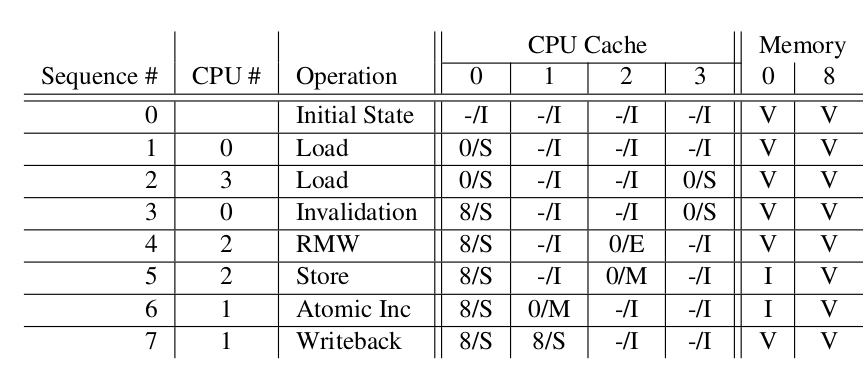
\includegraphics[width=0.5\textwidth]{./pics/mesi-sample.png}
\end{center}

\end{frame}


\begin{frame}[t,fragile]{Unnecessary stalls}

\begin{tikzpicture}[remember picture,overlay]
    \node[xshift=4.5cm,yshift=-7.5cm] at (current page.center) {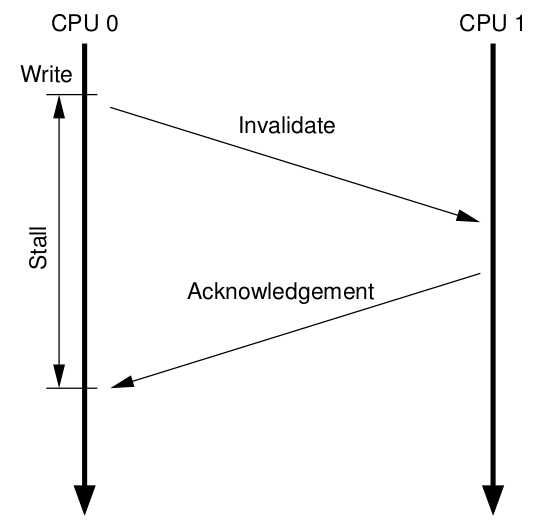
\includegraphics[width=0.4\textwidth]{./pics/stall.png}};
\end{tikzpicture}

\begin{itemize}
    \item CPU 0 starts write to cache line held by CPU 1
    \item CPU 0 must wait for the data to arrive
    \pause
    \item Why wait? CPU 0 is going to unconditionally overwrite it!
\end{itemize}

\end{frame}


\begin{frame}{Cache coherency: takeaways}

High-level ideas:
\begin{itemize}
    \item Memory split into chunks (cache lines) with auxiliary data (cache line state)
    \pause
    \item Copies of cache lines could reside in main memory and in processor-specific caches
    \pause
    \item Processors communicate via memory bus and use cache coherency protocol
    \pause
    \item Read/write operations change state of cache line and trigger message passing
\end{itemize}

\pause
Design choices:
\begin{itemize}
    \pause
    \item Cache line size (64, 128, 256 ...)
    \pause
    \item Number of states (MSI, MOESI, MESIF ...)
    \pause
    \item Hierarchy of caches (L1/L2/L3, iCache/dCache)
    \pause
    \item Topology of interconnect: see slide~\ref{interconnectPics}
    \pause
    \item When to send request? To whom? How to process incoming request?
\end{itemize}

\pause
Challenges:
\begin{itemize}
    \pause
    \item Invalidation storms
    \pause
    \item Unnecessary stalls 
\end{itemize}

\end{frame}

\section{Hardware optimizations} % Store Buffer, Invalidate Queue, Load Buffer
\showTOC

\begin{frame}{Concurrent invariants and where to violate them}

\begin{itemize}
    \item \textbf{Coherence}: in any execution, for each location, there is a single linear order of all writes to that location which must be respected by all threads
\end{itemize}

\begin{itemize}
    \item Step 1: "break" \ intuitive behaviour to get performance improvement
    \item Step 2: repair consistency
\end{itemize}
\end{frame}


\begin{frame}[t,fragile]{Which parts of cache coherence should be optimized?}

\begin{tikzpicture}[remember picture,overlay]
    \node[xshift=4cm,yshift=-4cm] at (current page.center) {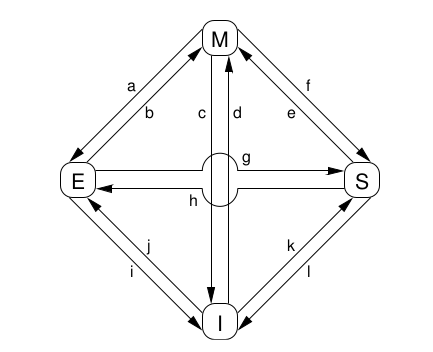
\includegraphics[width=0.5\textwidth]{./pics/MESI.png}};
\end{tikzpicture}


State machine:
\begin{itemize}
    \item \textbf{Modified}, \textbf{Exclusive}, \textbf{Shared}, \textbf{Invalid}
\end{itemize}

Message passing on some transitions:
\begin{itemize}
    \item asynchronous (fire and forget)
    \item synchronous (await confirmation)
\end{itemize}

Optimization opportunities:
\begin{itemize}
    \item Option 1: more states (MESIF, MOESI ...)
    \item \only<1>{Option 2: more asynchronous operations}\only<2>{\textbf{Option 2: more asynchronous operations}}
\end{itemize}

\end{frame}


\begin{frame}{Removing unnecessary stalls}

CPU execution:
\begin{itemize}
    \item \texttt{write(x = 1)} \pause \texttt{, cache\_line(x) is Shared}
    \pause
    \item Send invalidation requests \pause , Await confirmation
    \pause
    \item Modify \texttt{cache\_line(x)}

    \pause
    \item \texttt{write(y = 1)} \pause \texttt{, cache\_line(y) is Shared}
    \pause
    \item Send invalidation requests \pause ,  Await confirmation
    \pause
    \item Modify \texttt{cache\_line(y)}
\end{itemize}

\pause

\begin{tikzpicture}[remember picture,overlay]
    \node[xshift=4cm,yshift=-3cm] at (current page.center) {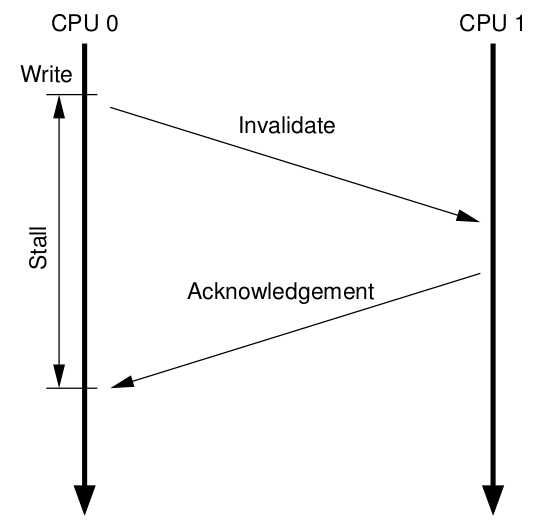
\includegraphics[width=0.4\textwidth]{./pics/stall.png}};
\end{tikzpicture}

\pause

Idea: batch processing
\begin{itemize}
    \item Buffer of "pending operations" \ that await confirmation
    \item Execute other instructions \textbf{before} invalidation confirmed
    \item Modification of the same location "consults" \ with buffer, not with cache (\textbf{store to load forwarding})
\end{itemize}

\end{frame}

\subsection{Store buffering}
\showTOCSub

\begin{frame}[fragile,t]{Store buffering}
 
 \begin{minted}[fontsize=\small]{c}
                           int x, y;
 \end{minted}
 
 \begin{tabular}{p{0.5\textwidth} p{0.5\textwidth}} 
 \begin{minted}[fontsize=\small]{c}
 void threadA() {
       x = 1;
   int a = y;
 }
 \end{minted}
 &  
 \begin{minted}[fontsize=\small]{c}
 void threadB() {                                   
         y = 1;                           
     int b = x;                           
 }                    
 \end{minted}
 \end{tabular}
 
 \pause
 
 \begin{tabular}{p{0.5\textwidth} p{0.5\textwidth}}
 \begin{minted}[fontsize=\small]{gas}
 # thread A
 mov [x] ,  1  # (A.1)
 mov EAX , [y] # (A.2)
 \end{minted}
 
 & 
 
 \begin{minted}[fontsize=\small]{gas}
 # thread B          
 mov [y] , 1  # (B.1) 
 mov EBX, [x] # (B.2) 
 \end{minted}
 \end{tabular}
 
 \end{frame}


 \begin{frame}[fragile,t,noframenumbering]{Store buffering}
 
 \begin{tabular}{p{0.5\textwidth} p{0.5\textwidth}}
 \begin{minted}[fontsize=\small]{gas}
 # thread A
 mov [x] ,  1  # (A.1)
 mov EAX , [y] # (A.2)
 \end{minted}
 
 & 
 
 \begin{minted}[fontsize=\small]{gas}
 # thread B          
 mov [y] , 1  # (B.1) 
 mov EBX, [x] # (B.2) 
 \end{minted}
 \end{tabular}
 
 \pause

What could we see in \texttt{(EAX EBX)}?

\only<1-4>{
 \texttt{\ \ \ \ \ \ \ \ \ \ \ \ \ \ \ \ \ \ \ \ \ \ (1 1)\ , (0 1)\ , (1 0)\ , (0 0)}
}
\only<5>{
 \texttt{Linearizable answer:\ \ (1 1)\ , (0 1)\ , (1 0)}
}
\only<6->{
 \texttt{Hardware answer:\ \ \ \ \ \ (1 1)\ , (0 1)\ , (1 0)\ , (0 0)}
}
\only<7->{
    \textbf{WHAT?}
}
 
 \pause
 Possible executions:
 \begin{itemize}
     \item \texttt{A.1 -> A.2 -> B.1 -> B.2}                               \only<4->{: \texttt{(0, 1)}}
     \item \texttt{\ \ \ \ \ \ \       B.1 -> A.2 -> B.2}                  \only<4->{: \texttt{(1, 1)}}
     \item \texttt{\ \ \ \ \ \ \ \ \ \ \ \ \ \              B.2 -> A.2}    \only<4->{: \texttt{(1, 1)}}
     \item \texttt{B.1 -> A.1 -> A.2 -> B.2}                               \only<4->{: \texttt{(1, 1)}}
     \item \texttt{\ \ \ \ \ \ \ \ \ \ \ \ \ \              B.2 -> A.2}    \only<4->{: \texttt{(1, 1)}}
     \item \texttt{\ \ \ \ \ \ \       B.2 -> A.1 -> A.2}                  \only<4->{: \texttt{(1, 0)}}
 \end{itemize}

\end{frame}
 


\begin{frame}[fragile]{Store buffering}

\begin{tikzpicture}[remember picture,overlay]
\node[xshift=4.5cm,yshift=-6.0cm] at (current page.center) {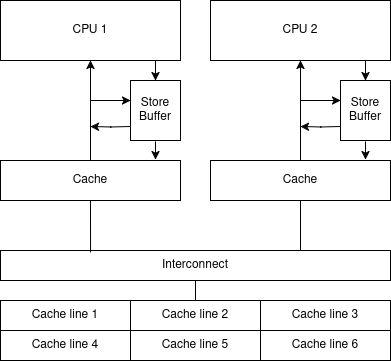
\includegraphics[width=0.35\textwidth]{./pics/processor/6.png}};
\end{tikzpicture}


 \begin{tabular}{p{0.32\textwidth} p{0.32\textwidth}}
 \begin{minted}[fontsize=\small]{gas}
 # thread A
 mov [x] ,  1  # (A.1)
 mov EAX , [y] # (A.2)
 \end{minted}
 
 & 
 
 \begin{minted}[fontsize=\small]{gas}
 # thread B          
 mov [y] , 1  # (B.1) 
 mov EBX, [x] # (B.2) 
 \end{minted}
 \end{tabular}

 \texttt{Hardware allows: (EAX=0 EBX=0)}

\begin{itemize}
    \item Looks like CPU reorders memory load and stores
    \item but does not break per-processor order \only<2>{\textbf{(store forwarding)}}
    \item and keeps cache coherency (linear order of writes for single memory location)
\end{itemize}

\end{frame}


\begin{frame}[fragile]{Store to load forwarding: why?}

\begin{center}
\begin{minted}{c}
      static int a = 0, int b = 0;
      a = 1;
      b = a + 1;
      assert(b == 2);
\end{minted}
\end{center}

\begin{itemize}
    \pause
    \item CPU 0: start execute \texttt{a = 1}, \texttt{a} not in cache
    \pause
    \item CPU 0: send "read invalidate"
    \pause
    \item CPU 0: put ''\texttt{write(a = 1)}'' to store buffer
    \pause
    \item CPU 1: receive ''read invalidate'', respond
    \pause
    \item CPU 0: start execute \texttt{b = a + 1}
    \pause
    \item CPU 0: receive cache line from CPU 1 (''\texttt{a} is zero''), put it to cache
    \pause
    \item CPU 0: use \texttt{a} value from cache (\texttt{a = 0})
    \pause
    \item CPU 0: commit ''\texttt{write(a = 1)}'' from store buffer (now cache thinks ''\texttt{a} is one'')
    \pause
    \item CPU 0: finish writing to \texttt{b} ('''\texttt{b} is one'')
    \pause
    \item CPU 0: assert failed
\end{itemize}

\pause

\begin{tikzpicture}[remember picture,overlay]
\node[xshift=4.5cm,yshift=0.0cm] at (current page.center) {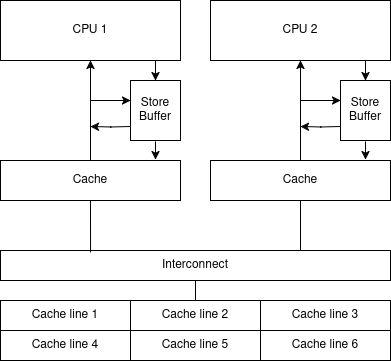
\includegraphics[width=0.35\textwidth]{./pics/processor/6.png}};
\end{tikzpicture}


\end{frame}

\begin{frame}{Store buffering: useful?}

\begin{itemize}
    \item Processor extended with internal buffer to speed-up execution
    \item In-processor order conforms to program order (\textbf{store forwarding})
    \begin{itemize}
        \item Perfect single-CPU abstraction
    \end{itemize}
    \item Other processor may see memory updates to happen in non-program order
    \begin{itemize}
        \item Abstraction leaks\footnote{\tiny\url{https://www.joelonsoftware.com/2002/11/11/the-law-of-leaky-abstractions/}} in multicore environment
    \end{itemize}
\end{itemize}

\pause
Some concurrent algorithms do not tolerate arbitrary memory reorderings (e.g. Peterson Lock).

\pause

How to repair them?

\pause

Use special CPU instruction:
\begin{itemize}
    \pause
    \item "flush store buffer before next operation"
    \pause
    \item "ensure no reordering of \textbf{this} and \textbf{that}"
    \pause
    \item "execute memory barrier instruction"
\end{itemize}

\pause

We will discuss few more hardware optimizations before diving into memory barriers.

\end{frame}


\subsection{Load buffering}
\showTOCSub

\begin{frame}[fragile]{Load buffering}

\begin{tikzpicture}[remember picture,overlay]
\node[xshift=4.5cm,yshift=-7.0cm] at (current page.center) {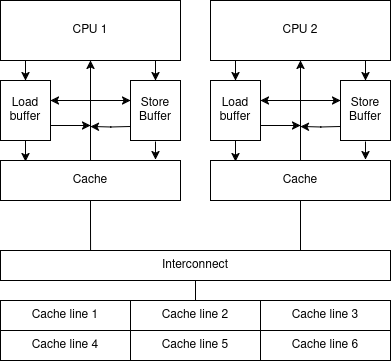
\includegraphics[width=0.35\textwidth]{./pics/processor/7.png}};
\end{tikzpicture}


 \begin{tabular}{p{0.32\textwidth} p{0.32\textwidth}}
 \begin{minted}[fontsize=\small]{gas}
 # thread A
 mov EAX , [y] # (A.1)
 mov [x] ,  1  # (A.2)
 \end{minted}
 
 & 
 
 \begin{minted}[fontsize=\small]{gas}
 # thread B          
 mov EBX, [x] # (B.1) 
 mov [y] , 1  # (B.2) 
 \end{minted}
\end{tabular}

\texttt{Possible result: (EAX=1, EBX=1)}

\pause

Some algorithms will fail (e.g. Peterson Lock).

\pause

How to repair them?

\pause

Use special CPU instruction:
\begin{itemize}
    \pause
    \item "flush load buffer before next operation"
    \pause
    \item "ensure no reordering of \textbf{this} and \textbf{that}" 
    \begin{itemize}
        \pause 
        \item should we flush load buffer and store buffer simultaneously?
    \end{itemize}
    \pause
    \item "execute memory barrier instruction"
\end{itemize}

\pause
Looks like we need different \textbf{kinds} of memory barriers.

\end{frame}


\subsection{Optional: Invalidate Queues}
\showTOCSub

\begin{frame}[fragile]{Invalidate Queue}

\begin{tikzpicture}[remember picture,overlay]
\node[xshift=4.5cm,yshift=-7.0cm] at (current page.center) {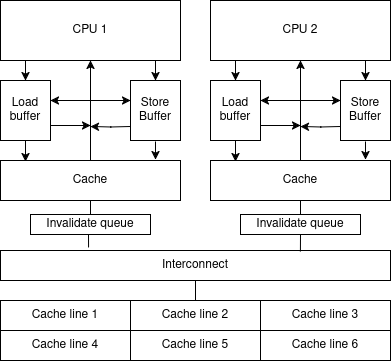
\includegraphics[width=0.35\textwidth]{./pics/processor/8.png}};
\end{tikzpicture}

\begin{minted}{c}
void foo(void) {
  a = 1;
  smp_mb(); // memory barrier
  b = 1;
}
void bar(void) {
  while (b == 0) continue;
  assert(a == 1); // fails with `a == 0`. WHAT?
}
\end{minted}

\pause
Key insight:
\begin{itemize}
    \item Synchronization is \textbf{always} a \textbf{communication}
    \begin{itemize}
        \item The one to initiate data exchange (writer, request sender)
        \item The one to ensure data view is consistent (reader, response sender)
    \end{itemize}
    \item "My thread executed strongest memory barrier, others will see updated data" \ is \textbf{NOT OK}
\end{itemize}

\end{frame}


\begin{frame}[t,fragile,noframenumbering]{Invalidate Queue}

\begin{tikzpicture}[remember picture,overlay]
\node[xshift=4.5cm,yshift=-7.0cm] at (current page.center) {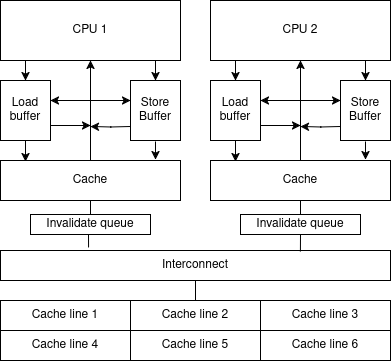
\includegraphics[width=0.35\textwidth]{./pics/processor/8.png}};
\end{tikzpicture}

\begin{minted}{c}
void foo(void) {
  a = 1;
  smp_mb(); // memory barrier
  b = 1;
}
void bar(void) {
  while (b == 0) continue;
  smp_mb(); // memory barrier
  assert(a == 1); // never fails
}
\end{minted}

Optional homework: perfbook.B.4.3

\end{frame}

\subsection{Interconnect topology}
\showTOCSub

\begin{frame}[t,fragile]{Independent Reads of Independent Writes}
 
 \begin{tabular}{p{0.2\textwidth} p{0.2\textwidth} p{0.2\textwidth} p{0.2\textwidth}}
 \begin{minted}[fontsize=\small]{python}
 thread1
   x = 1
 \end{minted}
 
 & 
 
 \begin{minted}[fontsize=\small]{python}
 thread2
   y = 1
 \end{minted}
 
 &
 
 \begin{minted}[fontsize=\small]{python}
 thread3
  r1 = x
  r2 = y 
 \end{minted}
 
 &
 
 \begin{minted}[fontsize=\small]{python}
 thread4
  r3 = y
  r4 = x
 \end{minted}
 \end{tabular}
 
 Assume there is no in-CPU reordering of memory operations (no load buffering)
 
 \pause
Is it possible to observe \texttt{(r1 = 1, r2 = 0, r3 = 1, r4 = 0)}?

\pause

\begin{center}
 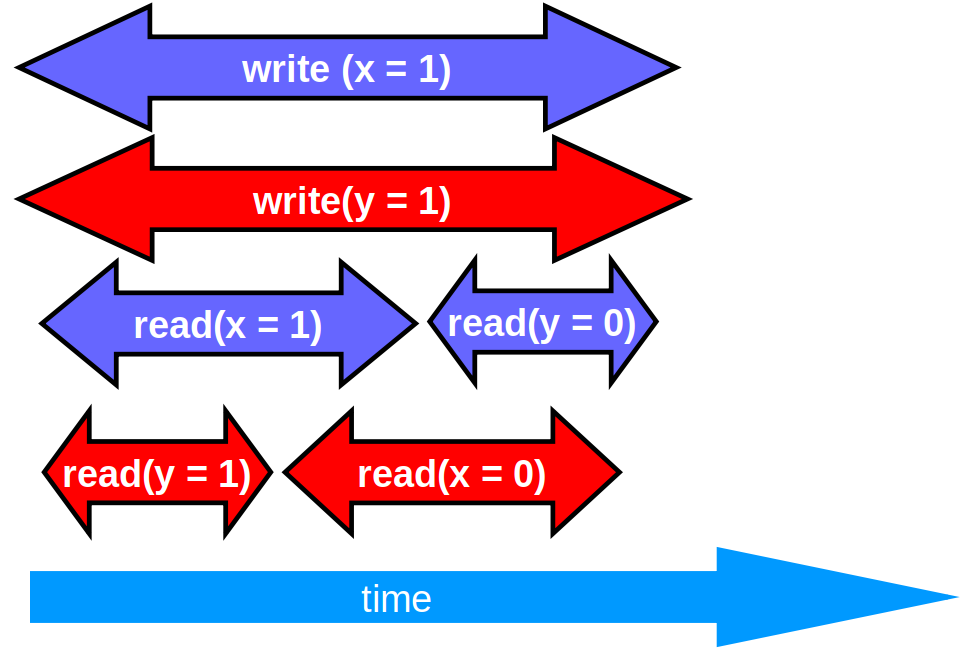
\includegraphics[width=0.35\textwidth]{./pics/iriw.png}
\end{center}

\end{frame}


\begin{frame}[t,fragile,noframenumbering]{Independent Reads of Independent Writes}
 
 \begin{tabular}{p{0.2\textwidth} p{0.2\textwidth} p{0.2\textwidth} p{0.2\textwidth}}
 \begin{minted}[fontsize=\small]{python}
 thread1
   x = 1
 \end{minted}
 
 & 
 
 \begin{minted}[fontsize=\small]{python}
 thread2
   y = 1
 \end{minted}
 
 &
 
 \begin{minted}[fontsize=\small]{python}
 thread3
  r1 = x
  r2 = y 
 \end{minted}
 
 &
 
 \begin{minted}[fontsize=\small]{python}
 thread4
  r3 = y
  r4 = x
 \end{minted}
 \end{tabular}
 
 Assume there is no in-CPU reordering of memory operations (no load buffering)

 Is it possible to observe \texttt{(r1 = 1, r2 = 0, r3 = 1, r4 = 0)}?

 Hint: it is NOT linearizable
 
 \pause
 \begin{itemize}
 \item \texttt{x86} or \texttt{x86\_64} (TSO): no
 
 \pause
 \item \texttt{ARM} or \texttt{POWER}: yes\footnote<3->{\tiny A Tutorial Introduction to the ARM and POWER Relaxed Memory Models, section 6.1}
 \end{itemize}
 
 \pause
 Information about cache lines could "travel" \ from one CPU to other CPU with different speed.

 \end{frame}


\begin{frame}[t,fragile,label={interconnectPics}]{Interconnect topology}

Key insight:
\begin{itemize}
    \item Cache lines could "travel" \ from one CPU to other CPU with different speed
\end{itemize}


\begin{tikzpicture}[remember picture,overlay]
\node[xshift=-4.5cm,yshift=-6.9cm] at (current page.center) {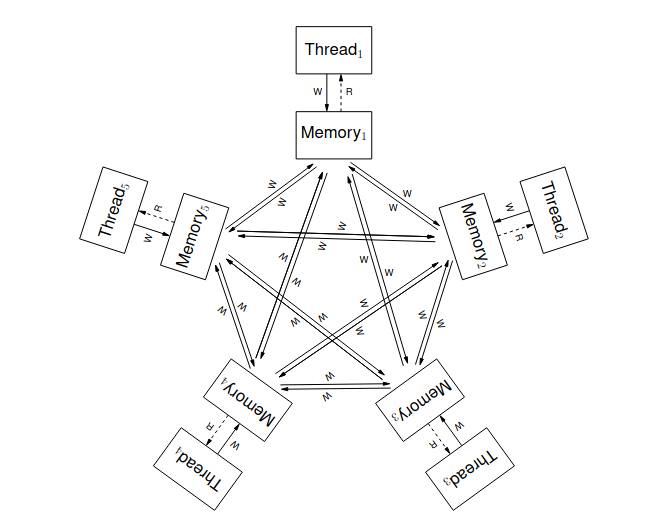
\includegraphics[width=0.45\textwidth]{./pics/interconnect1.png}};
\end{tikzpicture}

\begin{tikzpicture}[remember picture,overlay]
\node[xshift=2.5cm,yshift=-6.9cm] at (current page.center) {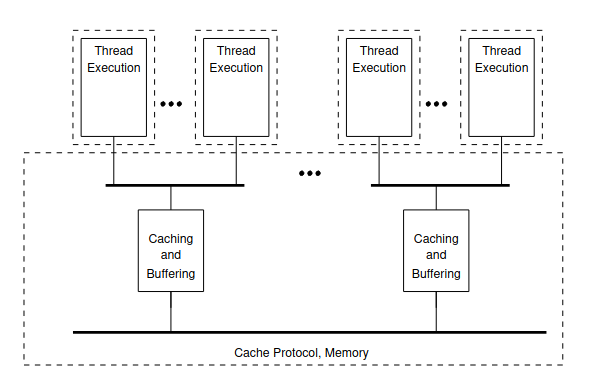
\includegraphics[width=0.45\textwidth]{./pics/interconnect2.png}};
\end{tikzpicture}

\end{frame}

\section{Hardware memory model}
\showTOC

\begin{frame}{Hardware-level reordering}

\only<1-2>{In one sentence}\only<3->{Conservative approximation}
\pause
\begin{itemize}
 \item Anything could be reordered with everything \only<4->{(point-of-view of some CPUs may disagree)}
 \pause
 \pause
 \pause
 \item Current CPU will "emulate" \ execution of single-threaded program "as if" \ in program order
 \pause
 \item Single memory cell is \textbf{coherent} 
 \begin{itemize}
    \pause
    \item linear order of writes for \textbf{particular} location
    \pause
    \item no ordering guarantees across \textbf{different} locations 
 \end{itemize}
\end{itemize}

\pause
How to treat non-synchronized memory accesses:
\begin{itemize}
    \pause
    \item Happened on some processor -- no guarantees it is visible on another processor
    \pause
    \item Synchronization is always a communication
    \begin{itemize}
        \pause
        \item somebody writes and ensures data will be properly shared (memory barrier)
        \pause
        \item somebody reads and ensures data view is consistent (memory barrier)
    \end{itemize}
    \pause
    \item "Today it works on my processor" \ is \textbf{NOT OK}
\end{itemize}

% For smarties
% - Caution: you could find \textbf{very few} exceptions to this rule (asymmetric dekker synhronization, linux membar, serialize via memaccess trap)  
%            actually, those are bi-directional algorithm
%            ask me why, if you are interested

\end{frame}


\begin{frame}[t,fragile]{Weak memory model}

We started with simplistic model of multiprocessor memory hierarchy

\pause

\begin{center}
  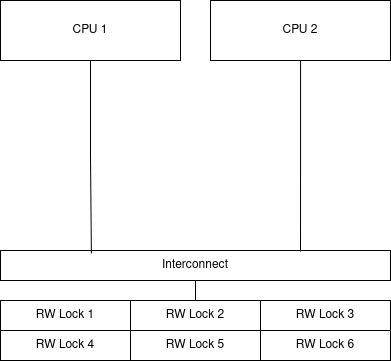
\includegraphics[width=0.3\textwidth]{./pics/processor/5.png}
\end{center}

\pause
\begin{itemize}
    \item All memory operations are guarded with read-write mutex (thus ordered)
    \item Read-mostly workloads scale quite well
    \item Performance is low due to contention and slow queries of data
\end{itemize}
\end{frame}


\begin{frame}[t,fragile,noframenumbering]{Weak memory model}

We started with simplistic model of multiprocessor memory hierarchy
\begin{itemize}
    \item All memory operations are guarded with read-write mutex (thus ordered)
    \item Read-mostly workloads scale quite well
    \item Performance is low due to contention and slow queries of data
\end{itemize}

\pause 
We started to optimize our model and lost "useful" \ consistency guarantees
\begin{itemize}
    \pause
    \item Replication pattern (multiple copies of same data in different caches)
    \pause
    \item Reordering of independent operations (store buffering, load buffering)
    \pause
    \item Making message-passing asynchronous (invalidate queues)    
    \pause
    \item Non-uniform interconnect (faster/slower message passing)
\end{itemize}

\end{frame}


\begin{frame}[t,fragile,noframenumbering]{Weak memory model}

We started to optimize our model and lost "useful" \ consistency guarantees
\begin{itemize}
    \item Replication pattern (multiple copies of same data in different caches)
    \item Reordering of independent operations (store buffering, load buffering)
    \item Making message-passing asynchronous (invalidate queues)    
    \item Non-uniform interconnect (faster/slower message passing)
\end{itemize}

\pause
We have less strict rules on what is guaranteed for memory operations
\begin{itemize}
    \item \textbf{Relaxed} memory model
    \item \textbf{Weak} memory model
\end{itemize}

\pause
\begin{itemize}
    \item Interesting fact №1: stronger CPU memory model -- less bugs you encounter during maintenance of large concurrent software system
    \item Interesting fact №2: smartphones, laptops, energy-efficient servers tend to use weak hardware
\end{itemize}

\end{frame}


\section{Memory barriers}
\showTOC

\begin{frame}{Memory barriers: definition}

\textbf{Memory barrier}
\begin{itemize}
    \item Hardware-specific machine instruction that helps to enforce some kind of ordering between memory operations 
    \pause
    \item Affects \textbf{current} processor
    \pause
    \item But actually we need to prevent reordering of memory operations \textbf{as they seen by other processors}
\end{itemize}
\pause
Do not forget to insert memory barriers on both sides of communication protocol!

\pause
Semantics is very architecture-specific:
\begin{itemize}
    \item \texttt{x86\_64}  -- \texttt{mfence}, \texttt{lock} prefix
    \item \texttt{arm64} -- \texttt{dmb}
    \item \texttt{power} -- \texttt{sync}, \texttt{lwsync}
\end{itemize}

\pause
Described in many pages of architecture manual. \pause Inconvenient.

\end{frame}


\begin{frame}[fragile]{Memory barriers: taxonomy}

\textbf{Memory barrier}
\begin{itemize}
    \item Hardware-specific machine instruction that helps to enforce some kind of ordering between memory operations 
    \item Affects \textbf{current} processor
    \item Should be used on both sides of communication protocol
\end{itemize}

\pause

Simplified taxonomy of memory barriers:
\begin{itemize}
    \item \texttt{Store\_Store}, \texttt{Store\_Load}, \texttt{Load\_Store}, \texttt{Load\_Load}
\end{itemize}

\pause

\begin{tabular}{p{8cm}p{5cm}}

\begin{minted}{c}
  int x = static.data1;
  Store_Store();
  Store_Load();
  int y = static.data2;
  static.data3 = 17;
\end{minted}

 &

 \begin{minted}{c}
  int x = static.data1;
  Load_Load();

  int y = static.data2;
  static.data3 = 17;
\end{minted}

\end{tabular}

\end{frame}


\begin{frame}{Memory barriers: rule of thumb}

\pause
Do not use them! \pause Seriously!

\pause

Every modern language supports civilized concurrency and provides plenty of useful tools:
\begin{itemize}
    \pause
    \item design-level abstractions -- \texttt{Executor}, \texttt{Future}, \texttt{ParallelStream} ... 
    \pause
    \item concurrent data structures -- \texttt{Lock}, \texttt{Semaphore}, \texttt{CountDownLatch}, \texttt{Monitor} ...
    \pause
    \item atomic read-modify-write operations - \texttt{getAndSet}, \texttt{compareAndExchange}, \texttt{getAndAdd} ...
\end{itemize}

\pause

Memory barriers are needed to:
\begin{itemize}
    \item implement basics (writing your own OS, compiler, VM)
    \pause
    \item get CRITICAL performance \pause and spend a lot of resources to maintain the code
    \pause
    \item design useful concurrent programming language (see you at next Lecture)
\end{itemize}

\end{frame}

\section{Litmus tests}
\showTOC

\begin{frame}[fragile]{Litmus test: definition}

\begin{itemize}
    \item \textbf{Litmus test}: very small concurrent program that access few shared variables and illustrates some relaxed-memory phenomena
\end{itemize}

\pause

\textbf{Coherence (CoRR1)}

Initial state: \texttt{x = 1}, Forbidden: \texttt{r1 = 2, r2 = 1}
\begin{tabular}{p{0.5\textwidth} p{0.5\textwidth}} 
 \begin{minted}[fontsize=\small]{c}
 void threadA() {
       x = 2;   
 }
 \end{minted}
 &  
 \begin{minted}[fontsize=\small]{c}
 void threadB() {                                   
     int r1 = x;                           
     int r2 = x;                           
 }                    
 \end{minted}
\end{tabular}

\pause

\textbf{Store buffering}

 \begin{tabular}{p{0.32\textwidth} p{0.32\textwidth}}
 \begin{minted}[fontsize=\small]{gas}
 mov [x] ,  1  # (A.1)
 mov EAX , [y] # (A.2)
 \end{minted}
 
 & 
 
 \begin{minted}[fontsize=\small]{gas}
 mov [y] , 1  # (B.1) 
 mov EBX, [x] # (B.2) 
 \end{minted}
 \end{tabular}

 \texttt{Hardware allows: (EAX=0 EBX=0)}

\end{frame}

\begin{frame}[fragile]{Litmus test}

Litmus tests are basic building blocks to construct reliable concurrent primitives

\begin{itemize}
    \pause \item Help to get "relaxed ordering" \ right
    \pause \item May be empirically checked against (new version of) hardware
    \pause \item Minimize "problematic surface" \ of concurrency library
    \pause \item Could be engineered as cross-platform functions (with different implementations)
    \pause \item Used to illustrate weak memory model related bug in complicated protocol\footnote<6->{\tiny ... this one bite us hard and scare the \%\$\^\! out of us \url{https://groups.google.com/g/mechanical-sympathy/c/QbmpZxp6C64}}\textsuperscript{,}\footnote<6->{\tiny Fix \url{https://github.com/torvalds/linux/commit/76835b0ebf8a7fe85beb03c75121419a7dec52f0}}
    \pause \item Could be used to provide non-portable yet highly efficient algorithms\footnote<7->{\tiny Section 4 "Linux x86 SpinLock implementation" \ in \url{https://dl.acm.org/doi/pdf/10.1145/1785414.1785443}}
    \pause \item Well-studied problem domain
\end{itemize}

\end{frame}


\section{Summary}


\begin{frame}{Summary}


Cache coherency
\begin{itemize}
    \item Cache line: granularity, false sharing, tagging with extra info    
    \item Cache coherency protocol: states, transitions, message passing, coherency
\end{itemize}

Hardware optimizations
\begin{itemize}
    \item Store buffering, Load buffering, Invalidate Queues, Interconnect topology
\end{itemize}

Hardware memory model
\begin{itemize}
    \item Reorderings of memory operations on independent memory locations
    \item Weak (relaxed) consistency
\end{itemize}

Memory barriers
\begin{itemize}
    \item Architecture-specific, Affect local CPU only, Different kinds
    \item \texttt{\{Store,Load\}\_\{Store,Load\}} taxonomy
\end{itemize}

Litmus tests
\begin{itemize}
    \item Basic blocks for many key concurrent algorithms
    \item Empirical approach to building reliable concurrent software    
\end{itemize}

\end{frame}


\begin{frame}{Summary: homework}

"Is Parallel Programming Hard, And, If So, What Can You Do About It" \ (perfbook) 

Appendix B "Why Memory Barriers?"

\begin{itemize}
    \item section B.1 ''Cache Structure''. Be ready to draw and explain what is associative hardware cache.
    \item section B.2.4 ''MESI Protocol Example''
\end{itemize}

\end{frame}



% \begin{frame}{Caches}
% 
% 1 cpu -- 1 cache + global memory
% 
% challenges: 
    % modified, how others will see
    % need to read -- from where?
    % need to write -- to which instance (local or remote?)
% 
% main requirements (informal)
    % per-cpu consistency
    % per-memory cell consistency
    % no-out-of-thin-air values (atomicity)
    % some "reasonable" causality (more on this later)
% 
% further reading: formal definition etc
% 
% \end{frame}
% 
% \begin{frame}{Cache coherency}
% 
% protocol that defines
% 
% who, when and how should write/read data and resolve "conflicts"
% 
% 
% for efficiency we use
    % data splitting (cache lines)
    % replication (severl CPUs may have a copy of main memory cacheline)
    % ownership (cacheline may be "exclusive" for this thread or read-only etc)
    % message passing (please transfer me a cahceline, please drop this cacheline as containing out-pf-date data)
    % asynchrony (I send message, do some stuff, receive answer and continue some stuff)
% 
% and that is why we get even MORE strange behaviour
% 
% IMPORTANT: as observer, everytihn looks like "operations are reorderd", "operations see out-of-date value", "no causality/transitivety in observed values"
% the same problem we already seen in compiler reordering but on really low level (even if your compiler is totally dumb)
% 
% Our goal here is to get a feeling of different problems and performance implications of h/w design.
% You MUST not use this models to reason about correctness of programs, NEVER
% 
% further reading: serios stuff on h/w mem models, tools, verifiers etc.
% \end{frame}
% 
% \begin{frame}{MESI protocol}
% 
% Not so simple, not so complicated
% 
% We have:
    % cachelines with states: semantics
    % transitions provoked by events (read write ext-message)
    % message send/receive policy
% 
% This protocol is used for illustration purposes, it is not used "as is" in serious h/w.
% 
% pictures, few scenarios
% 
% 
% Conclusion:
    % - replication works, if all read then it scales well
    % - contention on writes (real sharing), cache size explains "fake" mesasge invocations (false sharing)
    % - not only operation matters, side effects (triggered event) matter -- bus traffic/bus bandwith issues
% 
% some scenarios could be further tweaked, see MESIF as an example. 
% More states -- more messages and comlicated logic and more bits, but some scenarios could improve
% 
% 
% Ok, so far we already have some strange consistency behaviou (no linearizability granted, but per-cell consistency is ok)
% Remember how you suffered on various flavours of atomic-registers? Real life is harsh 
% 
% \end{frame}
% 
% 
% \begin{frame}{Store buffering}
% 
% Ok, we have some serious improvement on performance and scalability but our operations still need to be committed sequentially and we await a lot
% 
% what if we have some buffer of "operations to be done" and somehow do tasks "in parrallel" ?
% 
% Store buffer
% 
% Few caveats:
    % same location ops must be ordered or even joined
    % same location read-writes must be consistenct, stor-to-load buffering
% 
% This stuff now misbehaves on independent locations, we start to loose "transitivity" (and sanity).
% 
% And yes, you could observe it on modern intel/amd processors: see
% 
% 
% Sometime you need to "enforce" ordering, then use special CPU instruction "memory barrier".
% Incorrect but understandable definition "flush the buffer".
% Incorrect but "generic" definition: "forbid reordering of load and stores around this place in code"
% Incorrect but "mathematical" definition: add special "happens-before, proveds-afte, promising-inter" edges in concurency graph
% 
% Here you have seen approaches to h/w memory models:
% - operational
% - denotational
% - TODO
% 
% I intentioanlly use state-machine based explanation with diagrams and particular scenarios. It never helps to prove anything about code but could explain bugs/inconsistent behaviour. You should % understand it is "dangerous" stuff but not magic, just series of performance tradeoffs
% 
% further reading: habr
% 
% \end{frame}
% 
% \begin{frame}{Invalidation queue}
% 
% Ok, we traded "logical execution" in some scenarios (which were still possible to explain by compielr optimization for instrance) for better throughput
% what else is limiting our protocol?
% 
% awaiting confirmation from other cpu
% 
% lets use invalidation queue
% 
% diagram
% 
% even more subtle for correctness 
% 
% discuss few scenarios and problems
% 
% we need yet another memory barrier
% 
% \end{frame}
% 
% \begin{frame}{Note on memory barriers}
% 
% in general they are CPU specific instructions we some CPU specific semantics
% 
% but could be classified in classical
% StorStore/...
% 
% Golden RULE:
% abundant barriers on one side do not guarantee correctness on other side, for proper comunication you need barriers (or other sync ops) on both sides
% 
% You should not think
% SL\_SL barrier publishes everthing and now it is visible
% or atomic.sseqcst in C++ or volatile in Java or Atomic in Java
% 
% any commujnication is 2-way process (send message, receive message)
% 
% \end{frame}
% 
% \begin{frame}{Load buffer}
% 
% Ok, speeding up stuff. Lets buffer independent loads
% 
% diagram
% 
% even more comlicated scenario
% 
% yes indeed it happens on arm64, see litmus
% 
% but buys us simplicity/perfomance/energy efficiency
% 
% \end{frame}
% 
% \begin{frame}{Cache topology}
% 
% By the way, how information about cahe state is moved around
% physically, over wire
% but who sends to whom
% 
% diagram with single arbiter
% diagram with n-way topology
% 
% here are scenario that also illustrate some strange "transitivity violation"
% 
% \end{frame}

% \begin{frame}{Hardware is evolving}
% 
% new cache coherency protocols will appear
% new modules (buffers, reorders, predictors, queues ...) will appear
% topology and rules of memory bus functioning will change
% 
% so this "operational view" illustrtion is already outdated.
% 
% But key points are:
% - replication indeed works and may be a game changer in scalability/performance
% - reorderings are possible and happen all the time, no matter bacuase of compiler or hardawre or memory bus specific
% 
% You need to know how to tame the beast.
% 
% Evil way (knut):
% - memory barriers
% - syncing atomic operations
% 
% Good way (prianik)
% - thread- or cpu-specific data
% - read-mostly applications
% 
% Rule of thumb: if you are desperately getting "yet one more clock cycle" by using ultra-advanced concurrent algorithm with "on-the-edge" weakest-allowed memory-barriers
% maybe you are solving the task wrong way
% 
% - it is hard to validate
% - it is hard to maintain
% - it is very h/w specific and will be outdated soon
% 
% In some sense, you are great multicore developer if you are not using 2/3 of this course in production code
% 
% Unfortunately, personal experience of many cool concurrency experts shows that first you need to learn hard stuff and spend (A LOT OF) time debugging it
% 
% \end{frame}


% \begin{frame}{Hardware memory model}
% 
% All this operational stuff and scenario anecdotes are cool but they indeed do not help us to prove programs are OK
% 
% And processor manuals are also hard to interpret in terms of concurrent code.
% What should we do?
% 
% 
% Answer #1: mathematics!
% Use formalism to describe properties, orderings, guarantees and then prove comlicated propositions of assembly snippets
% 
% See introduction to relaxed memoty models
% see adve
% 
% Pros: real math
% Cons: not for daily use
% 
% Answer #2: reuse!
% somebody implemts mutex for you and you just use it as is. maube author even proves some stuff about the code
% Pros: i tried to teach you this way in block1
% Cons: how to develop custom algos?
% 
% further reading: how they optimized spin lock on x86 for linux by removing some barrier
% 
% Answer #3: litmus tests!
% you write small snippets about communication between threads, ensure they work as intended and build algos of this small briks
% Pros: flexible
% Cons: need deep knowledge of caveats, time conusming, suboptimal
% 
% Please read about taxonomy of tests, use special software to study this.
% 
% Warning:
%     there are well established hardware memory models for differnt archs
%         but they still find "imprecisions" there (russ cox link about arm-whatever)
%     under these models is possible to prove behaviour of moderate asm snippets
%         - not large chinks
%         - not high level code (becase verifying compiler optimizations agains memory model is other story) 
% 
% \end{frame}



\end{document}
